
\documentclass[runningheads,a4paper]{llncs}

\usepackage[utf8]{inputenc}            % kodowanie
\usepackage[OT4]{fontenc}              % font PL
\usepackage[polish]{babel}
% \usepackage{amssymb}
% \usepackage{minted}
\usepackage{listings}
\usepackage{color}
\setcounter{tocdepth}{3}
\usepackage{graphicx}
\usepackage{epstopdf}
\usepackage{caption}
\captionsetup{compatibility=false}
\captionsetup{justification=centering}
\usepackage{subcaption}
\setcounter{secnumdepth}{3}

\definecolor{mygreen}{rgb}{0,0.6,0}
\definecolor{mygray}{rgb}{0.5,0.5,0.5}
\definecolor{mymauve}{rgb}{0.58,0,0.82}
\definecolor{mygrey}{rgb}{0.97,0.97,0.97}

\lstset{
  backgroundcolor=\color{mygrey},   % choose the background color; you must add \usepackage{color} or \usepackage{xcolor}
  basicstyle=\footnotesize\ttfamily,        % the size of the fonts that are used for the code
  breakatwhitespace=false,         % sets if automatic breaks should only happen at whitespace
  breaklines=true,                 % sets automatic line breaking
  captionpos=b,                    % sets the caption-position to bottom
  aboveskip=0pt,
  abovecaptionskip=0pt,
  commentstyle=\color{mygreen},    % comment style
  deletekeywords={...},            % if you want to delete keywords from the given language
  escapeinside={\%*}{*)},          % if you want to add LaTeX within your code
  extendedchars=true,              % lets you use non-ASCII characters; for 8-bits encodings only, does not work with UTF-8
%   frame=single,                    % adds a frame around the code
  framexleftmargin=3pt,
  framexbottommargin=3pt,
  framextopmargin=0pt,
  framexrightmargin=3pt,
  framerule=0.1pt,
  keepspaces=true,                 % keeps spaces in text, useful for keeping indentation of code (possibly needs columns=flexible)
  keywordstyle=\color{blue},       % keyword style
%   morekeywords={*,...},            % if you want to add more keywords to the set
  numbers=left,                    % where to put the line-numbers; possible values are (none, left, right)
  numbersep=8pt,                   % how far the line-numbers are from the code
  numberstyle=\footnotesize\color{mygray}, % the style that is used for the line-numbers
  rulecolor=\color{black},         % if not set, the frame-color may be changed on line-breaks within not-black text (e.g. comments (green here))
  showspaces=false,                % show spaces everywhere adding particular underscores; it overrides 'showstringspaces'
  showstringspaces=false,          % underline spaces within strings only
  showtabs=false,                  % show tabs within strings adding particular underscores
  stepnumber=1,                    % the step between two line-numbers. If it's 1, each line will be
  stringstyle=\color{mymauve},     % string literal style
  tabsize=4,                       % sets default tabsize to 2 spaces
  title=\lstname                   % show the filename of files included with \lstinputlisting; also try caption instead of title
}

\usepackage{float}
\usepackage[justification=centering]{caption}

\floatstyle{plain}
\newfloat{glastopf_listing}{bhp}{}[section]
\floatname{glastopf_listing}{Listing}

\usepackage{url}
\urldef{\mailsa}\path|{alfred.hofmann, ursula.barth, ingrid.haas, frank.holzwarth,|
\urldef{\mailsb}\path|anna.kramer, leonie.kunz, christine.reiss, nicole.sator,|
\urldef{\mailsc}\path|erika.siebert-cole, peter.strasser, lncs}@springer.com|
\newcommand{\keywords}[1]{\par\addvspace\baselineskip
\noindent\keywordname\enspace\ignorespaces#1}

\renewcommand{\keywordname}{\textbf{Słowa kluczowe:}}

\setlength{\fboxsep}{0pt}
\setlength{\fboxrule}{1pt}

\begin{document}

\mainmatter
\title{Wykrywanie ataków w sieciach komputerowych z wykorzystaniem systemów Honeypot}
\author{Maciej Jagiełło}

\titlerunning{ }
\authorrunning{ }
\institute{}
\maketitle

\begin{abstract}
Artykuł opisuje projekt architektury sieci honeypotów przeznaczonej do wykrywania ataków sieciach komputerowych. Opisane są popularne honeypoty użyte w systemie. Przedstawione są narzędzia do wdrażania systemu. Zamieszczony jest krótki opis aplikacji oraz pokazane są bliźniacze projekty.
\keywords{honeypot, glastopf, kippo, dionaea, vagrant, puppet, virtualbox}
\end{abstract}


\section{Wprowadzenie}

Wykrywanie ataków w sieciach komputerowych to ważny element działań na rzecz zwiększania bezpieczeństwa systemów. Cyberprzestępczość rozwija się szybkim tempem. Z każdym dniem opracowywane są nowe sposoby ataków, wykorzystywane są nowe podatności w aplikacjach, protokołach i systemach operacyjnych. Aby temu przeciwdziałać, konieczne jest opracowanie odpowiednich narzędzi.

Celem systemu jest stworzenie narzędzia do zbierania adresów IP\footnote{To taki adres np. 127.0.0.1, który identyfikuje komputer w sieci.} hakerów, botów\footnote{Programy, które wykonują coś automatycznie. Najczęściej są instalowane przez hakerów jako wirusy, ale mogą być też uruchamiane z jego osobistego komputera.} i zainfekowanych maszyn\footnote{Bardziej ogólna nazwa dla komputera} w spójną bazę danych\footnote{Taka baza danych to najczęściej tabela wyglądająca jak w Excelu.}, którą będzie można później wykorzystać np. do rozszerzania reguł zapór ogniowych\footnote{ang. firewall - zatrzymuje niechciane połączenia do komputera. Jedna z prostszych metod przeciwdziałania atakom. Domyślnie instalowany w Windowsach}. System ma być też źródłem nowych wirusów do analizowania przez antywirusy. Wybrane rozwiązanie problemu to sieć Honeypotów\footnote{ang. Garnek z miodem. Taka atrapa do łapania hakerów}.

Honeypot to jedynie idea zbierania informacji. Jest to kombinacja ustawień sprzętowych i programowych, które tworzą system pułapkę. Ustawienia sprzętowe, czyli komputer, wyodrębniony obszar sieci lokalnej, który odpowiednio symuluje prawdziwą sieć, ale jest od niej odizolowany i zabezpieczony.

Taki system, uruchomiony na maszynie serwerowej\footnote{Maszyna serwerowa to po prostu komputer}, udostępnia w Internecie jakiś zasób atrakcyjny dla atakującego. Może to być rekord w bazie danych, aplikacja lub cały system operacyjny. Używając odpowiednich mechanizmów do monitorowania zachowania, zbiera dane o sposobach wykonywania ataków.

Jego główną zaletą jest to, że korzystają z niego niemal wyłącznie użytkownicy, którzy chcą włamać się do sieci.

Aby z sukcesem doprowadzić do wdrożenia i utrzymania takiego systemu niezbędne są technologie wspomagające wdrożenie\footnote{Wdrożenie polega na instalacji i konfiguracji aplikacji gdzieś na jakimś serwerze}. Przedstawione zostaną one w kolejnych rozdziałach artykułu. Działający system, który dostarcza już dane, będzie mógł je prezentować w formie przyjaznej dla człowieka. Ta część systemu przedstawiona zostanie na przykładzie podobnych projektów.

\section{Sieć honeypotów}

Na rysunku \ref{fig:architektura_fig} przedstawiony jest schemat architektury aplikacji. Każdy honeypot uruchomiony jest w maszynie wirtualnej\footnote{Maszyna wirtualna to system operacyjny w systemie operacyjnym.}. Maszyna ta posiada dostęp do Internetu i wystawia do niego, odpowiednie dla zainstalowanych honeypotów, zasoby. Moduł pobierania i analizy logów zbiera pozostawione przez honeypoty informacje o atakujących. Są to ślady wykonywanych akcji i pliki binarne\footnote{Pliki binarne (przeciwieństwo to pliki tekstowe) to pliki, których się nie czyta, bo są skompresowane i reprezentowane jako bajty, a nie jako litery} ładowane na maszyny przez atakujących.

\begin{figure}
        \centering
        \fbox{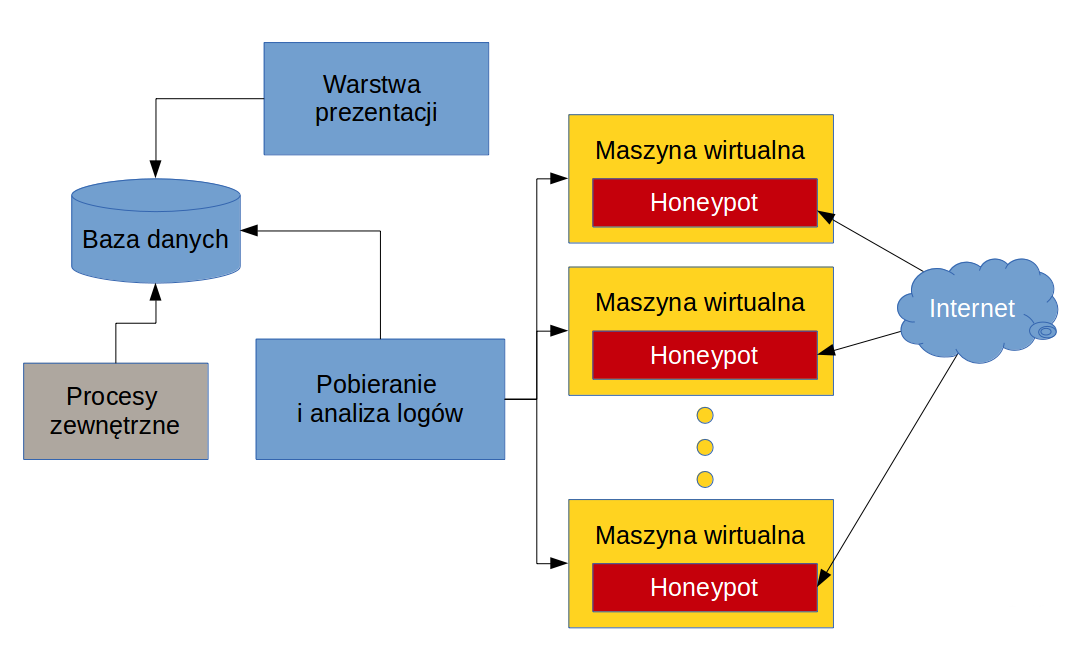
\includegraphics[width=1.0\textwidth]{pics/architektura}}
        \caption{Architektura aplikacji.}
        \label{fig:architektura_fig}
\end{figure}

Istnieje bardzo dużo realizacji honeypotów. Na stronie \cite{honeynet_project}, która zajmuje się rozwojem narzędzi do zwiększenia bezpieczeństwa w Internecie, jest wymienione około 30 projektów, a to z pewnością nie wszystkie dostępne.

Warto wspomnieć o pracującym na wydziale Elektroniki i Technik Informacyjnych\footnote{Mój wydział}, doktorze Krzysztofie Cabaju, który na przedmiotach BSS, SKM2 i TKOM prowadzi studentów podczas implementacji\footnote{Implementacja to popularne słowo na pisanie aplikacji} autorskich honeypotów.

W opisywanym systemie zostały wybrane trzy realizacje honeypotów ze względu na wystarczającą różnorodność w oferowanych przez nie usługach.

\section{Honeypoty}

\subsection{Glastopf}
Pierwszy z prezentowanych honeypotów, Glastopf\footnote{niem. Szklany garnek}, jest zwykłą stroną www, którą można znaleźć w wyszukiwarkach internetowych. Treść strony zawiera frazy w języku angielskim, które są generowane z dostarczonej przez twórców bazy danych. Glastopf potrafi w prosty sposób analizować zapytania HTTP\footnote{Gdy wejdziesz na stronę google.pl, to tak naprawdę wyślesz zapytanie GET protokołem HTTP do serwera o domenie google.pl.}, w szczególności te zapytania GET, które w adresie URL zawierają inne adresy URL do zewnętrznych plików. Takie argumenty parsuje\footnote{Analizuje jego znaczenie. Tekst dla komputera jest niezrozumiały póki nie będzie wiedzieć jak go czytać. Parsowanie to proces, który zamienia jeden ciąg literek w inne struktury danych} i próbuje ściągać na dysk do późniejszej analizy.

\subsection{Kippo}

Kolejnym wektorem ataków, na jaki są podatne komputery w sieciach komputerowych jest protokół\footnote{Protokołem do stron internetowych jest HTTP.} ssh\footnote{Protokół do zdalnego wykonywania komend w konsoli na komputerze}. Kippo symuluje sesję SSH udostępniając prostego shella\footnote{Aplikacja do uruchamiania komend}. Najczęściej używane polecenia mają napisane własne implementacje, które oszukują użytkownika tego środowiska\footnote{Atakujący musi myśleć, że jest na prawdziwym komputerze, a nie na atrapie}. Polecenia rzadziej używane zwracają błąd, w taki sposób, aby nie zdradzić fałszywości systemy. Kippo udostępnia dla nich fałszywy system plików\footnote{To co zaczyna się od C: w Windowsie} tylko do odczytu, który wygląda jak po świeżej instalacji Debiana\footnote{System operacyjny typu Linux}.

Ta aplikacja loguje informacje o adresach IP, próbach pobrania plików z Internetu, zapisuje te pliki w kwarantannie, oraz loguje całą sesję użytkownika od próby zalogowania na serwer, aż do aktywności po wylogowaniu. Robi to przechwytując polecenia „logout“, „exit“ lub znak wysyłany kombinacją klawiszy Ctrl + D. Następnie wyświetla znak zachęty\footnote{Znak, który oznacza, że konsola oczekuje kolejnego polecenia} wyglądający jak na lokalnym komputerze.

\subsection{Dionaea}

Ostatnim z użytych w systemie honeypotów jest Dionaea. Protokoły, którymi się posługuje do serwowania pułapki to głównie Samba, HTTP, FTP, MySQL, RTP. Samba jest bardzo popularnym protokołem do wymiany plików w Windowsie. Wiele osób bez zaawansowanej wiedzy o tym systemie korzysta z niego i nieumyślnie otwiera sobie drogę do włamania. Dlatego atakujący często szukają drogi właśnie tym kanałem.

\section{Środowisko uruchomieniowe}

Istotnym, choć niekoniecznym krokiem w stronę bezpieczeństwa systemu jest uruchamianie serwerów honeypotowych w maszynie wirtualnej. Pozwala to osiągnąć wysoki poziom separacji środowiska podatnego na ataki, od rzeczywistej maszyny, nad którą nie można stracić dostępu. Dodatkowo to rozwiązanie jest bardzo przydatne gdy jest potrzeba, by system był łatwy w replikacji na inne maszyny. Aplikacja uruchamiająca maszynę wirtualną jest odpowiedzialna za dostarczenie takiego samego środowiska. W opisywanym systemie tą aplikacją jest VirtualBox rozwijany przez firmę Oracle.

Dodatkową warstwą nad VirtualBoxem jest Vagrant. Jest to świetne narzędzie do automatyzacji instalacji maszyny wirtualnej z użyciem skryptów konfiguracyjnych\footnote{Skrypt konfiguracyjny to jakaś aplikacja}. Jego użycie polega na przygotowaniu skryptu instalacyjnego\footnote{Znów aplikacja} na naszej maszynie. W tym systemie do instalacji honeypotów został użyty Puppet. Puppet to narzędzie do deklaratywnego\footnote{Deklaratywny sposób to pisanie jaki ma być stan, czyli CO ma być zrobione. Np. woda ma być ugotowana. Przeciwieństwo - imperatywny sposób - to pisanie JAK ma coś być zrobione np. wstaw wodę i zacznij gotować aż osiągnie 100 st. C.} zarządzania stanem\footnote{Zainstalowanymi aplikacjami, stworzonymi plikami} maszyny.

Alternatywą do wirtualnej maszyny jest wirtualny kontener\footnote{Sam nie wiem co to jest :)}, który nie tworzy wirtualnego systemu od początku do końca, a tylko izoluje aplikację od systemu. Najpopularniejszym rozwiązaniem jest Docker. Docker potrzebuje mniej zasobów systemowych\footnote{Procesor, Dysk, Ram}, ale nie gwarantuje 100\% bezpieczeństwa.

\subsection{Narzędzia}

Wartym do wejścia w szczegóły tematem jest wspólne działanie Vagranta, VirtualBoxa i Puppeta. Schemat jest przedstawiony na rysunku \ref{fig:vagrant_fig}. Numery obok strzałek oznaczają kolejne kroki instalacji honeypota na maszynie wirtualnej.

\subsection*{Vagrant i VirtualBox}

Zanim można rozpocząć procedurę, należy pobrać dystrybucję\footnote{Konkretną wersję systemu operacyjnego. Np. wspomniany Debian} systemu poleceniem:
\begin{lstlisting}
$ vagrant init hashicorp/precise32
\end{lstlisting}

Następnie polecenie \texttt{vagrant up} uruchamia procedurę. Najpierw Vagrant, korzystając z VirtualBoxa tworzy wirtualne środowisko. Potem uruchamia skrypty Puppetowe. One instalują się na maszynie tworząc gotowe środowisko.

Dostęp do stworzonej maszyny można uzyskać poprzez polecenie \texttt{vagrant ssh}.

\begin{figure}
        \centering
        \fbox{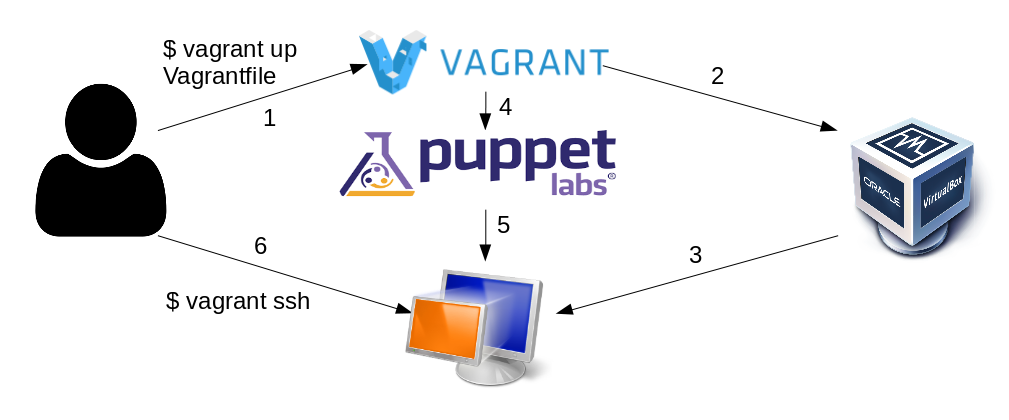
\includegraphics[width=1.0\textwidth]{pics/vagrant}}
        \caption{Vagrant, Puppet, VirtualBox.}
        \label{fig:vagrant_fig}
\end{figure}

Cały proces trwa około 5 minut, został wykonany z użyciem 3 poleceń w terminalu\footnote{Inaczej konsola}, a wynikiem jest maszyna wirtualna z ubuntu server w 32 bitowej wersji z zainstalowanym honeypotem.

\subsection*{Puppet}

Przykładowy i skrócony na potrzeby artykułu plik puppetowy jest na listingu \ref{glastopf_file}.

\begin{glastopf_listing}[h]
\lstinputlisting[language=Octave,caption={glastopf.pp},label={glastopf_file}]{code/glastopf.pp}
\end{glastopf_listing}

W skrypcie puppetowym w sposób deklaratywny określa się jak ma wyglądać stan maszyny po instalacji. Istnieje wiele wbudowanych modułów\footnote{Bibliotek, które tak naprawdę są kolejnymi aplikacjami}, które pozwalają zarządzać plikami, serwisami, aplikacjami, skryptami do uruchomienia, itp. Do zbioru modułów można doinstalowywać te udostępnione przez społeczność. A w nich są takie, które np. zarządzają gitem\footnote{Aplikacja do śledzenia zmian w plikach podczas pisania programów, tak, żeby jak coś się przypadkiem usunie, żeby dało się do tego wrócić.}.

Do uruchomienia skryptu z listingu \ref{glastopf_file} potrzebujemy tylko jednego polecenia:
\begin{lstlisting}
$ puppet apply glastopf.pp
\end{lstlisting}
Podczas wykonywania tego polecenia, Puppet analizuje plik \texttt{pp} i interpretuje go z użyciem modułów. Moduły wbudowane są napisane w języku Ruby i mogą być przygotowane dla różnych systemów operacyjnych. To, który się wykona zależy od środowiska, które rozpozna Puppet.

\section{Aplikacja}

Silnik do zbierania danych to aplikacja napisana w języku Java. Jego działanie polega na logowaniu się na serwer za pomocą protokołu SSH i pobraniu logów\footnote{Plików tekstowych z wpisami, które zostawił honeypot}. To gdzie się one znajdują jest zdefiniowane dla każdego honeypota oddzielnie. Na metadane\footnote{Metadane to dane o danych} o każdym z honeypotów składają się:
\begin{itemize}
\item lista lokalizacji plików do ściągnięcia,
\item reguły rozpoznawania plików tekstowych.
\end{itemize}

Aplikacja archiwizuje i utrwala pobrane dane w bazie danych. Analizuje ona również aktywność atakujących wg reguł zdefiniowany w metadanych, tak aby wyciągnąć adres IP komputera wysyłającego atak, stempel czasowy ataku i jego typ. Dane te później agreguje i udostępnia w formie zrozumiałej dla warstwy prezentacji, tak jak na rysunku \ref{architektura_fig}.

Jednym z problemów przy pobieraniu logów jest to, że ze względów bezpieczeństwa honeypot nie powinien mieć dostępu do żadnej części tworzonego systemu, ponieważ w przypadku włamania się na serwer, haker może zniszczyć nie tylko maszynę z honeypotem.

Zostało to rozwiązane właśnie używając protokołu SSH. Nie wymaga on instalowania dodatkowych aplikacji, wspiera przesyłanie plików i jest protokołem względnie bezpiecznym w porównaniu do innych autorskich rozwiązań.

Kolejnym problemem, który można spotkać podczas używania i konserwacji systemu jest rosnący bez końca plik z logami. Aby sobie z tym poradzić należy go okresowo archiwizować i usuwać, jeśli przekroczy określony rozmiar. Użyta została do tego aplikacja dostępna w repozytorium Ubuntu - logrotate.

Testy integracyjne aplikacji zostały wsparte przez technologie użyte przy wdrażaniu honeypotów: Vagrant, Virtualbox i Puppet.

\section{Warstwa prezentacji}

Istnieje kilka systemów dostępnych w Internecie, którym dane do prezentacji mógłby dostarczać system przedstawiony w artykule.

Pierwszym z nich jest Norse - IPViking Live, którego wygląd pokazany jest na rysunku \ref{fig:norse_fig}. Przedstawia on mapę świata, na której wyświetlane są ataki na żywo. Jego atrakcyjność zwiększona jest przez dynamikę aktualnych ataków, niestety niemożliwej do przedstawienia na jednym rysunku.

\begin{figure}
        \centering
        \fbox{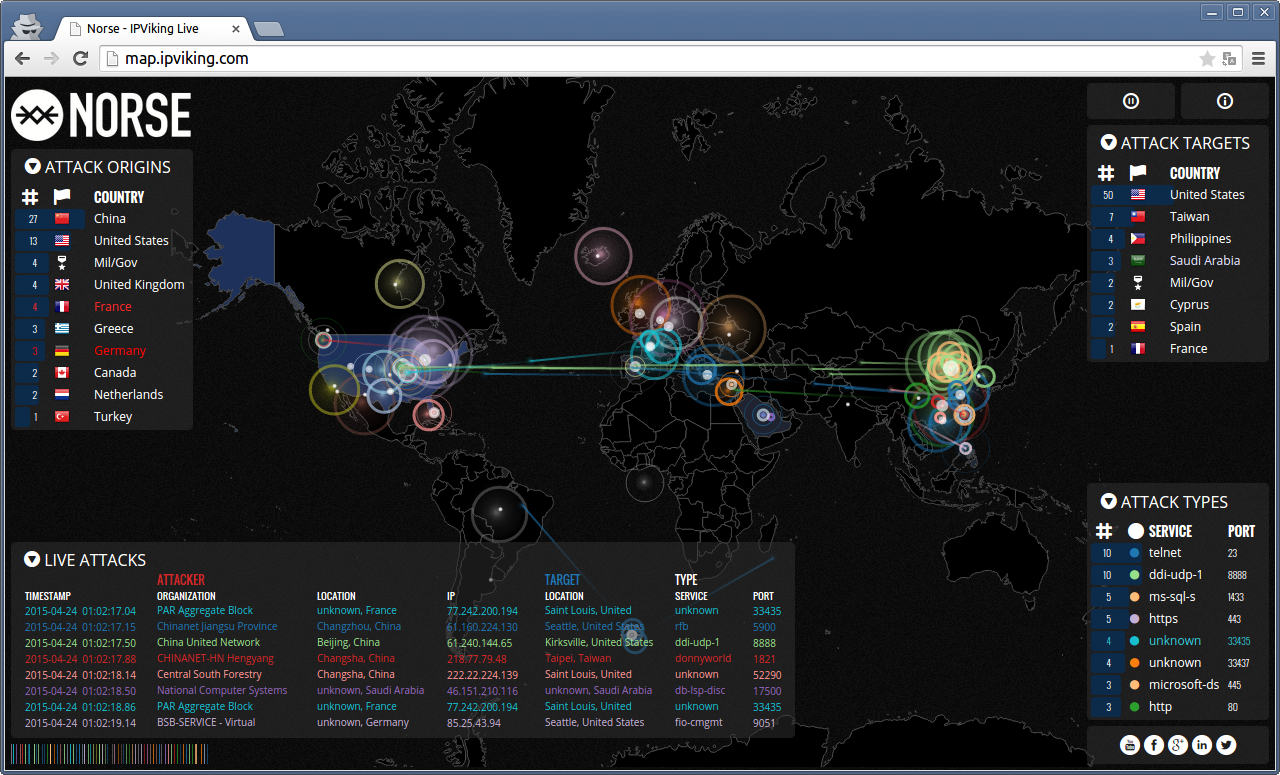
\includegraphics[width=1.0\textwidth]{pics/norse}}
        \caption{Norse – IPViking Live.}
        \label{fig:norse_fig}
\end{figure}

Nie istnieje wiele kluczowych różnic od drugiej mapy ataków, pokazanej na rysunku \ref{fig:digitalattackmap_fig}, którą powołał do życia Google ideas, Big Picture Group, a dane dostarcza Arbor Networks. Z pewnością niewiele danych jest wspólnych między tymi dwoma projektami. Skala ataków jest na tyle duża, że nie sposób tego kontrolować w sposób pełny.

\begin{figure}
        \centering
        \fbox{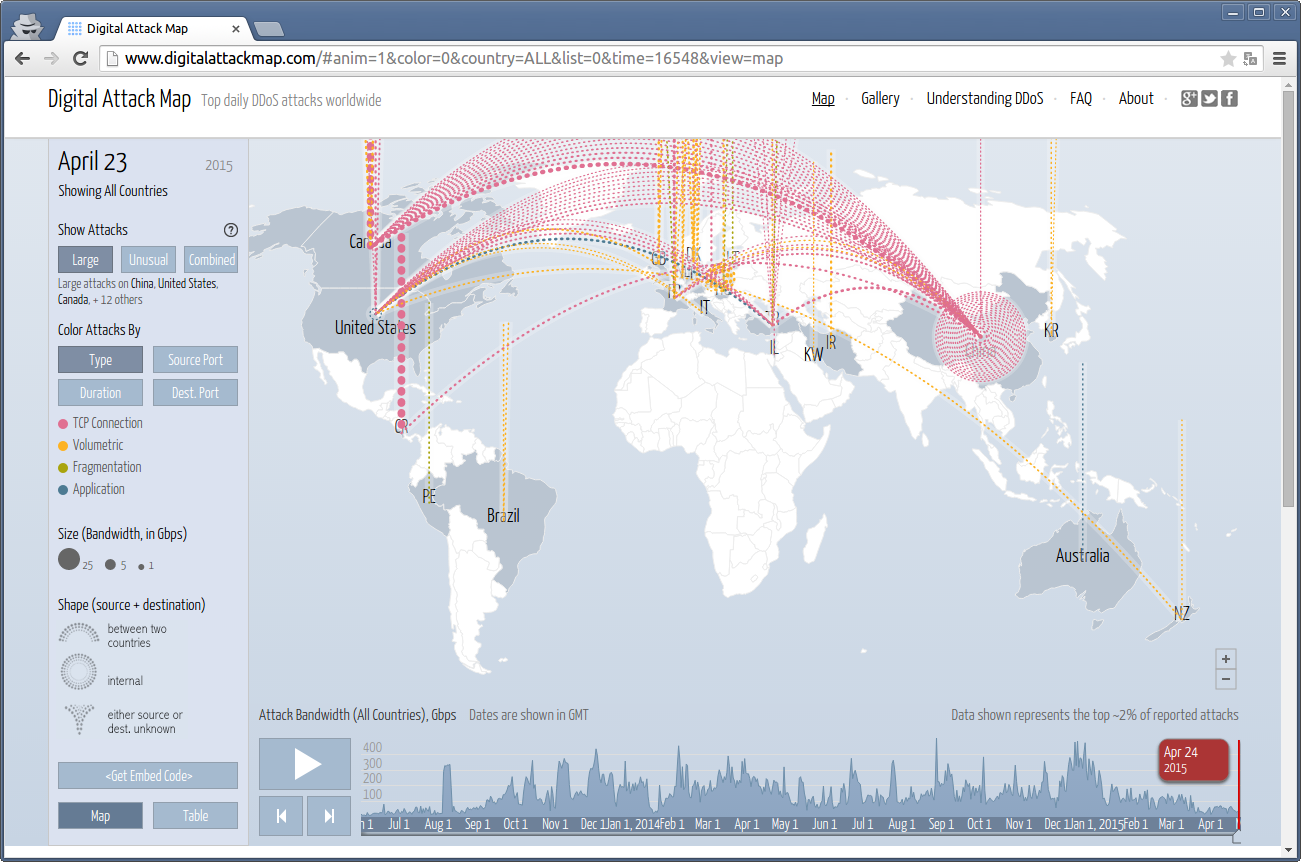
\includegraphics[width=1.0\textwidth]{pics/digitalattackmap}}
        \caption{Digital Attack Map.}
        \label{fig:digitalattackmap_fig}
\end{figure}

\section{Podsumowanie}

Do wykonania systemu wykrywającego ataki w sieciach komputerowych został użyty system honeypotów. Wdrażany przy użyciu technologii Vagrant, VirtualBox, Puppet i Java. Użyte honeypoty to Glastopf, Dionaea i Kippo, które oczekiwały na atakujący z użyciem protokołów HTTP, SSH, FTP, MySQL i RTP.

Pierwsze dane od botów skanujących internet pojawiły się już po paru dniach. Po kilku tygodniach średnia liczba ataków na jeden honeypot to 50 ataków na godzinę.

Boty atakujące serwer Glastopf najczęściej posiadały w nagłówku zapytania\footnote{Np. przeglądarki internetowe w nagłówku wysyłają to jaką są przeglądarką, jaka jest ich wersja, jaka jest wersja systemu operacyjnego} informację, że to tylko zbieranie danych na potrzeby badań edukacyjnych. Jednak rzeczywistość każe sądzić, że to tylko próba odwrócenia uwagi od faktycznego ataku.

\begin{thebibliography}{1}

% \bibitem{url} Xa,
% \url{http://xa}

\bibitem{} \url{http://jbeczala.republika.pl/files/ataki_sieciowe.pdf}
\bibitem{honeynet_project} \url{https://www.honeynet.org/project}
\bibitem{} \url{http://glastopf.org/}
\bibitem{} \url{https://github.com/desaster/kippo}
\bibitem{} \url{https://www.honeynet.org/project}
\bibitem{} \url{http://map.ipviking.com/}
\bibitem{} \url{http://digitalattackmap.com/}
\bibitem{} \url{https://puppetlabs.com/}
\bibitem{} \url{https://www.virtualbox.org/}
\bibitem{} \url{https://www.vagrantup.com/}
\bibitem{} \url{http://www.digitalforreallife.com/2012/11/boosting-teamwork-with-vagrant/}


\end{thebibliography}

\end{document}
